\documentclass[10pt, a4paper]{article}
\usepackage[utf8]{inputenc}
\usepackage{amsmath}
\usepackage{amssymb}
\usepackage{amsthm}
\usepackage{parskip}
\usepackage{enumitem}
\usepackage{siunitx}
\usepackage{tikz}
\usepackage{pgfplots}
\usetikzlibrary{arrows.meta}
\pgfplotsset{compat = newest}

\title{Física Contemporánea\\Resolución de Tarea 1}
\author{Vite Riveros Carlos Emilio\\ Romero De La Rosa Gabriela Michelle\\ 
        Fisher Bautista Emir Julián\\ López Gallegos Fátima}
\date{23 septiembre del 2022}

\begin{document}
    \maketitle
    1. Problemas
    \begin{enumerate}
        \item El vector $\vec{a}$ tiene las componentes $(8, 14, 4)$ unidades respectivamente:
        
        \begin{center}
            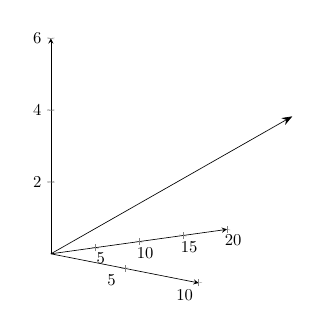
\begin{tikzpicture}[scale=.6]
                    \begin{axis}[
                        xmin=0, 
                        xmax=10, 
                        ymin=0, 
                        ymax=20, 
                        zmax=6,
                        zmin = 0, 
                        axis lines = middle,  
                        view = {50}{10}]
                        \addplot3[
                            -{Stealth[scale=1.3]}]table
                        {
                            x   y   z
                            0   0   0
                            8   14  4
                            
                        };
                    \end{axis}
            \end{tikzpicture}
        \end{center}
        
       \begin{enumerate}
            \item Obtenga la expresión del vector $\vec{a}$ en términos de los vectores unitarios.
            \item Determine una expresión para un vector $\vec{b}$ de $\frac{1}{4}$ de la longitud de $\vec{a}$ 
            apuntando en la misma dirección de $\vec{a}$.
            \item Calcule una expresión en términos de los vectores unitarios para un vector de
            tres veces la longitud de $\vec{a}$ apuntando en la dirección opuesta a la de él.
       \end{enumerate}
       \item Un automóvil viaja hacia el Este con una rapidez de $50 \si{\frac{km}{h}}$. Está lloviendo
       verticalmente con respecto a la Tierra. Las marcas de la lluvia sobre las ventanas
       laterales del automóvil forman un ángulo de 60 grados con la vertical, calcule la
       velocidad de la lluvia con respecto a: (a) el automóvil y (b) la Tierra.
       \item Dos remeros en canoas idénticas ejercen el mismo esfuerzo remando en un río,
       uno corriente arriba (y se mueve corriente arriba), mientras que el otro rema
       directamente corriente abajo. Un observador en reposo sobre la orilla del río
       determina sus rapideces, $V_1$ y $V_2$ respectivamente. Determine, en términos de
       los datos conocidos, la rapidez del agua en el río.
    \end{enumerate}
\end{document}
